\addchap{Die Fakultät Informatik}

Der \emph{Andreas-Pfitzmann-Bau} (kurz: APB, häufig auch einfach \glqq{}Fak\grqq{} genannt ), das Gebäude welches die Fakultät Informatik beherbergt, wird in den nächsten 3 bis 5 Jahren euer zweites Zuhause werden.
Viele Lehrveranstaltungen und Übungen werden hier stattfinden und mit zunehmender Semesterzahl werdet ihr immer weniger über den Campus gescheucht und immer mehr Veranstaltungen werden hier stattfinden. 
Doch was hat dieser Bau eigentlich zu bieten außer einer Menge grüner Farbe und der Skulptur im Foyer?
Darum soll es in diesem Kapitel gehen!

Der wesentliche Unterschied zwischen diesem Gebäude und den anderen auf dem Campus ist, das es rund um die Uhr geöffnet ist. Auch wenn nachts mal die Türen verschlossen sein sollten, wird euch der Nachtwächter gerne gegen Vorlage eures Studentenausweises die Tür öffnen und auf Wunsch auch einen der Seminarräume im Erdgeschoss aufschließen. Nur die PC-Pools bleiben euch zu nächtlicher Stunde verwehrt.
Einer nächtlichen Lernorgie sollte trotzdem nichts im Wege stehen. ;)

Außerdem können wir einen ziemlich schicken Außenbereich unser Eigen nennen. Mit Teich, viel Platz auf der Wiese zum rumlümmeln und Außensteckdosen, die den Energiebedarf eines Informatikers voll Schaffenskraft mühelos stillen können.

Eine Menge Sitzgelegenheiten auf den Gängen aller Etagen bieten euch auch in der Prüfungsphase genügend Platz, um euch mit euren Lerngruppen auf die anstehenden Prüfungen vorzubereiten. Das \texttt{ascii} wird gerne euren Koffeinbedarf stillen.

% TODO: Bild vom Teich hier


\pagebreak

% TODO: Change this to minisec? Adjust formatting for more :sparkle:? Same for Games Night!
\addchap{ascii - Das Café in der Fakultät}

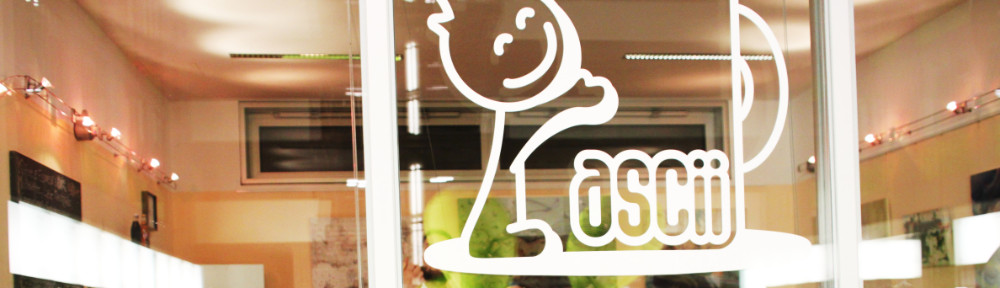
\includegraphics[width=\linewidth]{img/ascii.jpg}

Bereits seit 2007 existiert im Gebäude der Fakultät Informatik das ascii, ein Café betrieben von Studenten für Studenten, Mitarbeiter und Besucher, kurzum: für jeden.
Das ascii hat alles was ein richtiges Café so braucht: Kaffee, Kuchen, Bagels so wie alles was Nerds an der Fakultät so brauchen: Koffeinhaltige Kaltgetränke!
Zudem zählt das ascii zu den wenigen Adressen auf dem Campus, in denen man neben Club Mate auch Kolle Mate und Premium Cola erhält.
Hinter dem Tresen stehen Studenten, die gerne an einem Tag in der Woche noch ein paar Stündchen ihrer Freizeit zur Verfügung stellen.

Das ascii wird von einem studentischen Verein betrieben und ist seit seiner Gründung eine zentralen Anlaufstelle für jede und jeden an der Fakultät.
Hier treffen sich Studenten, Mitarbeiter und Professoren um ihre Pausen zu verbringen,
zu arbeiten oder einfach ihren Koffeinhaushalt aufzufüllen.
Auf den gemütlichen Sofas kann man die Zeit wunderbar an sich vorbei streichen lassen,
gemeinsam an Projekten arbeiten, lernen, programmieren oder einfach nur mit seinen Kommilitonen plaudern.
Du kennst noch niemanden an der Fakultät?
Du hast Fragen oder Gesprächsbedarf?
Wenn du ins ascii kommst, wirst du schnell sehen, dass an dem Vorurteil, Nerds seien nicht sozial, absolut nichts dran ist.

Wenn du jetzt Lust bekommen hast, das ascii zu besuchen oder sogar als Mitglied selbst mitzumachen, dann komm doch einfach mal vorbei und sag Hallo!

Weitere Hinweise findest du auf \link{http://www.ascii-dresden.de/}.

\textit{Wir öffnen in der Vorlesungszeit Montag bis Donnerstag von 9 bis 17 Uhr und Freitags von 9 bis 15 Uhr. Dazwischen sind wir aber auch häufig im Café anzutreffen.}

\pagebreak

\addchap{Spieleabende}

Einmal im Monat wird in der Fakultät vom FSR ein Spieleabend ausgerichtet. Start ist dabei immer um 18:30 Uhr im Foyer. Dabei stellt der FSR sein umfangreiches Angebot an analogen Spielen zur Verfügung, sodass eine ganze Menge an Spielen schon von Haus aus da sind. Wollt ihr etwas spielen, was nicht da ist, bringt es am besten mit! Oft sind auch schnell Leute gefunden, die mal ein neues Spiel ausprobieren wollen.

Hin und wieder finden sich auch ein paar Leute, die an dem Abend ihre Notebooks mitbringen und eine kleine LAN-Party schmeißen oder ihre Spielekonsole mitbringen, um über einen der Beamer der Seminarrunde mit anderen zusammen zu spielen.

Für Knabbereien und Getränke ist gesorgt, das ascii hat in der Regel zu Spieleabenden geöffnet. Wenn das Wetter mitspielt, ist auch das \emph{Count Down}, ein Dresdner Studentenclub, zur Stelle und verkauft Heißes vom Grill sowie alkoholische Getränke.

Es lohnt sich also auf jeden Fall, einmal vorbei zu schauen!

% TODO: Image

\pagebreak 

\
\thispagestyle{empty}
\AddToShipoutPicture*{\put(0,0){%
\parbox[b][\paperheight]{\paperwidth}{%
\vfill
\centering
\refstepcounter{dummy}
\label{spieleabendplakat}
\includegraphics[width=\dimen107,height=\dimen108,keepaspectratio]{img/spieleabend.png}%
\vfill
}}}

